\chapter{Исследовательская часть}

\section{Технические характеристики}

Технические характеристики устройства, на котором выполнялись замеры по времени:

\begin{itemize}
	\item Процессор: Apple M1 Pro \cite{m1}
	\item Оперативная память: 32 ГБайт.
	\item Операционная система: macOS Ventura 13.5.2. \cite{macOS}
\end{itemize}

При замерах времени ноутбук был включен в сеть электропитания и был нагружен только системными приложениями.

\section{Демонстрация работы программы}

На изображении \ref{img:demonstration} представлена иллюстрация работы разработанного программного продукта. 
Конкретно, демонстрируются результаты выполнения алгоритмов сортировки.
\clearpage
\begin{figure}[h]
	\centering
	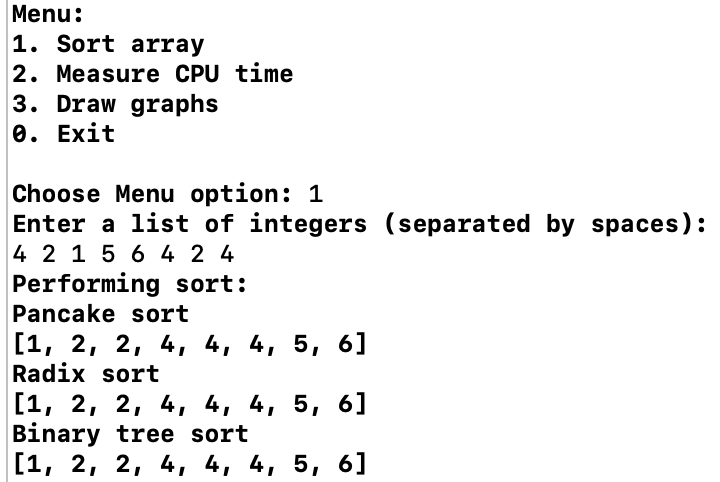
\includegraphics[height=0.4\textheight]{img/example.png}
	\caption{Демонстрация работы программы}
	\label{img:demonstration}
\end{figure}

\clearpage
\section{Анализ временных характеристик}

В данном разделе представлены результаты экспериментов, в которых измерялось время выполнения сортировок. 
Данные результаты представлены в таблицах \ref{tbl:sorted}, \ref{tbl:backSorted} и \ref{tbl:random}.

Таблица \ref{tbl:sorted} содержит результаты замеров времени выполнения алгоритмов сортировки для отсортированного входного массива размером в диапазоне от 1 до 901 с шагом 10.

\begin{table}[ht]
	\small
	\begin{center}
		\begin{threeparttable}
		\caption{Результаты замеров времени (массив уже отсортирован)}
		\label{tbl:sorted}
		\begin{tabular}{|c|c|c|c|}
			\hline
			& \multicolumn{3}{c|}{\bfseries Время, мкс} \\ \cline{2-4}
			\bfseries Размер массива & \bfseries Блинная & \bfseries Поразрядная & \bfseries Бинарным деревом
			\csvreader{csv/sorted.csv}{} 
			{\\\hline \csvcoli & \csvcolii & \csvcoliii & \csvcoliv} \\
			\hline
		\end{tabular}	
		\end{threeparttable}
	\end{center}
\end{table}

На основе данных из таблицы \ref{tbl:sorted} был построен график (см. рисунок \ref{plt:sorted}).
\clearpage

\begin{figure}[h]
	\centering
	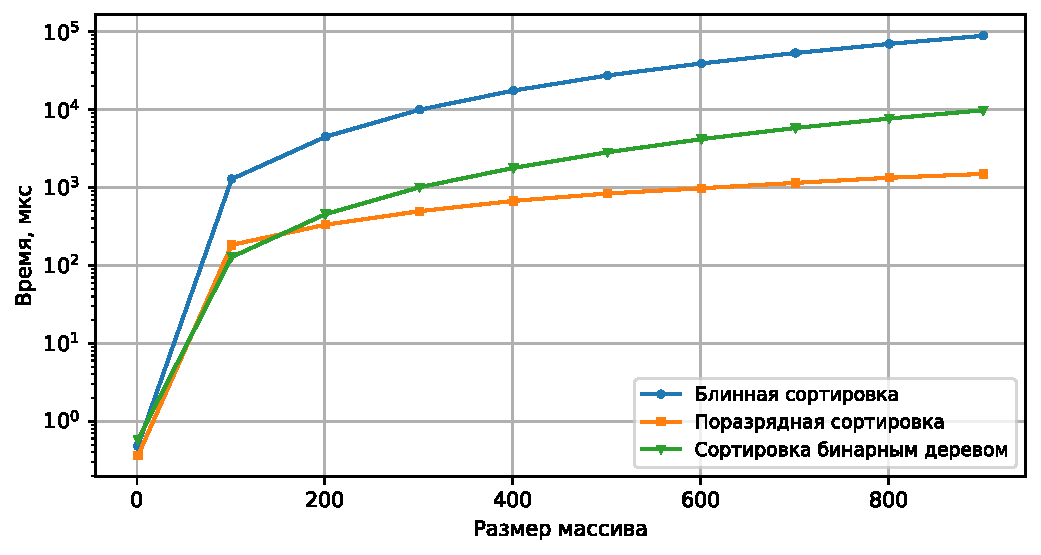
\includegraphics[height=0.3\textheight]{img/sorted.pdf}
	\caption{Сравнение времени выполнения алгоритмов сортировки для отсортированного массива}
	\label{plt:sorted}
\end{figure}

Таблица \ref{tbl:backSorted} содержит результаты замеров времени выполнения алгоритмов сортировки для массивов, отсортированных в обратном порядке.
\begin{table}[ht]
	\begin{center}
		\begin{threeparttable}
		\small
		\caption{Результаты замеров времени (массив отсортирован в обратном порядке)}
		\label{tbl:backSorted}
		\begin{tabular}{|c|c|c|c|}
			\hline
			& \multicolumn{3}{c|}{\bfseries Время, мкс} \\ \cline{2-4}
			\bfseries Размер массива & \bfseries Блинная & \bfseries Поразрядная & \bfseries Бинарным деревом
			\csvreader{csv/backSorted.csv}{}
			{\\\hline \csvcoli & \csvcolii & \csvcoliii & \csvcoliv} 
			\\
			\hline
		\end{tabular}
		\end{threeparttable}
	\end{center}
\end{table}

На основе данных из таблицы \ref{tbl:backSorted} был построен график (см. рисунок \ref{plt:backSorted}).

\begin{figure}[h]
	\centering
	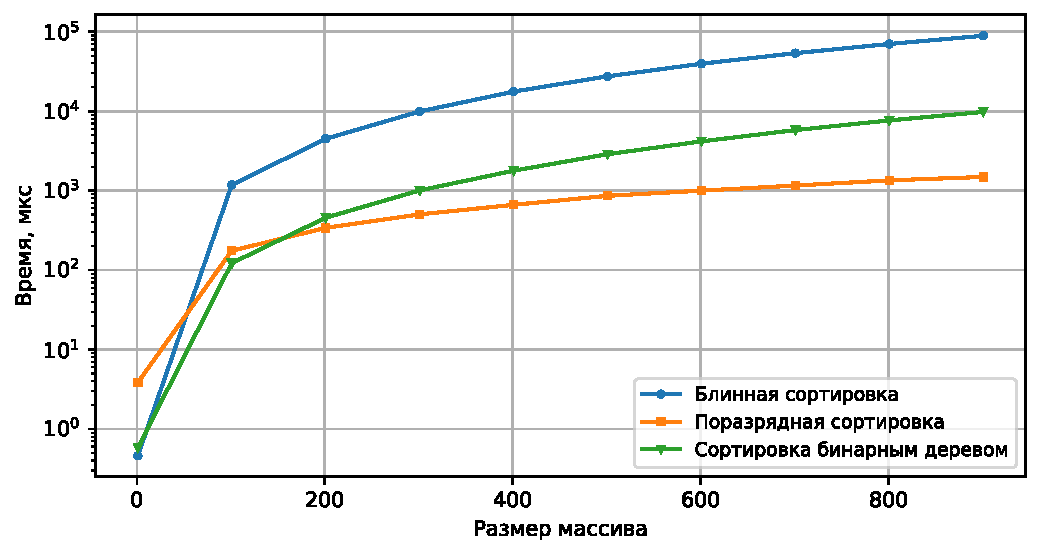
\includegraphics[height=0.3\textheight]{img/backSorted.pdf}
	\caption{Сравнение времени выполнения алгоритмов сортировки для массивов, отсортированных в обратном порядке}
	\label{plt:backSorted}
\end{figure}
\newpage

Таблица \ref{tbl:random} содержит результаты замеров времени выполнения алгоритмов сортировки для массивов, содержащих случайный набор данных.
\clearpage
\begin{table}[ht]
	\begin{center}
		\begin{threeparttable}
		\small
		\caption{Результаты замеров времени (случайный набор данных)}
		\label{tbl:random}
		\begin{tabular}{|c|c|c|c|}
			\hline
			& \multicolumn{3}{c|}{\bfseries Время, мкс} \\ \cline{2-4}
			\bfseries Размер массива & \bfseries Блинная & \bfseries Поразрядная & \bfseries Бинарным деревом
			\csvreader{csv/random.csv}{}
			{\\\hline \csvcoli & \csvcolii & \csvcoliii & \csvcoliv} 
			\\
			\hline
		\end{tabular}
		\end{threeparttable}
	\end{center}
\end{table}

На основе данных из таблицы \ref{tbl:random} был построен график (см. рисунок \ref{plt:random}).

\begin{figure}[h]
	\centering
	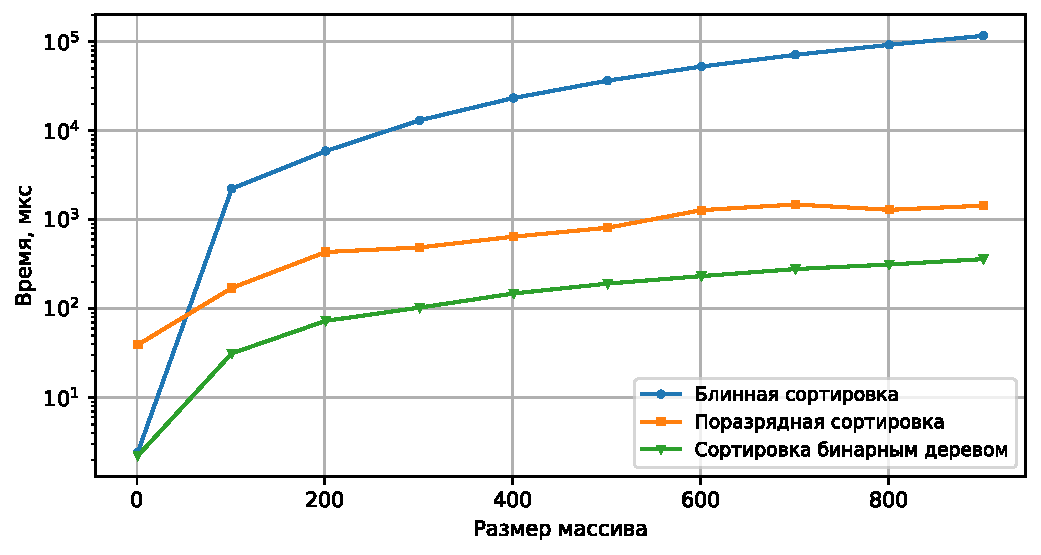
\includegraphics[height=0.3\textheight]{img/random.pdf}
	\caption{Сравнение времени выполнения алгоритмов сортировки для массивов, содержащих случайные наборы данных}
	\label{plt:random}
\end{figure}
\newpage

\section{Выводы}
Исходя из полученных результатов, сортировка бинарным деревом на отсортированных массивах и блинная сортировка на случайном массиве показывают наименьшую эффективность (на длине массива в 800 элементов примерно в 71 раз дольше, чем поразрядная сортировка), при этом поразрядная сортировка показала себя лучше всех на любых данных.
Можно сделать вывод, что использование сортировки бинарным деревом показывает наилучший результат при случайных, никак не отсортированных данных, т.к. при отсортированных данных обычное бинарное дерево вырождается в связный список, из-за чего вырастает высота дерева. 
Поразрядная сортировка же эффективнее в том случае, когда заранее известно максимальное количество разрядов в сортируемых данных.

Теоретические результаты оценки трудоёмкости и полученные практическим образом результаты замеров совпадают.